\documentclass[11pt,a4paper]{article}

\usepackage[utf8]{inputenc}
\usepackage[T1]{fontenc}
\usepackage{lmodern}
\usepackage[margin=0.95in]{geometry}
\usepackage{amsmath,amssymb}
\usepackage{booktabs}
\usepackage{graphicx}
\usepackage{xurl}
\usepackage{hyperref}
\usepackage{xcolor}
\usepackage{microtype}
\usepackage{enumitem}

\hypersetup{
  colorlinks=true,
  linkcolor=blue!60!black,
  citecolor=blue!60!black,
  urlcolor=teal!70!black,
  pdftitle={CRISOL-MBA-x64: Certified Neuro-Symbolic Deobfuscation of x86-64 Machine-Code Slices via Hybrid CEGIS and Lean 4 bv\_decide},
  pdfauthor={Luis Alejandro Arancibia}
}

\title{\textbf{CRISOL-MBA-x64: Certified Neuro-Symbolic Deobfuscation of x86-64 Machine-Code Slices via Hybrid CEGIS and Lean 4 \texttt{bv\_decide}}}

\author{
  Luis Alejandro Arancibia\\
  \textit{Computer Engineer (FIUBA, University of Buenos Aires)}\\
  \textit{Independent Researcher --- CrisoLabs Research Lab}\\
  ORCID: \href{https://orcid.org/0009-0003-6453-575X}{0009-0003-6453-575X}\\
  \texttt{arancibialuisalejandro@gmail.com}
}

\date{November 2026}

\begin{document}
\maketitle

\begin{abstract}
Mixed Boolean-Arithmetic (MBA) obfuscation remains a primary barrier in binary reverse engineering, malware analysis, and security auditing. Algebraic simplifiers such as SiMBA, GAMBA, ProMBA, and RUMBA achieve high speed on pure expression trees, yet fail when obfuscation is compiled into real x86-64 machine code entangled with carry-flag propagation (\texttt{ADC}/\texttt{SBB}), 32-to-64-bit zero-extension, arithmetic shifts (\texttt{SAR}), and bit rotations (\texttt{ROL}/\texttt{ROR}). Conversely, neural approaches such as LLM4Decompile and gMBA operate on string expressions or evaluate only finite test-case re-executability without universal formal guarantees, exposing analysts to silent edge-case hallucinations.

We present \textbf{CRISOL-MBA-x64}, a certified neuro-symbolic deobfuscation framework that pairs LLM candidate synthesis with a zero-LLM-trust verification pipeline that is sound relative to the declared Trusted Computing Base (TCB): a minimalist x86-64 lifter empirically cross-checked on 1,024 concrete vectors against native x86-64 execution and Unicorn (0 discrepancies across 82,944 three-way checks covering 31 instruction unit tests, 28 dataset-sanity slices, and all 22 \texttt{V\_real} slices), a vectorized concrete pre-filter, dual \texttt{QF\_BV} SMT solvers (Bitwuzla + Z3), and independently checked \textbf{LRAT} SAT proof certificates (\texttt{CaDiCaL} + \texttt{lrat-check}) as well as \textbf{Lean 4 \texttt{bv\_decide}} proof certificates that verify bit-blasting inside Lean.

Following a pre-registered anti-leakage protocol with disjoint identity families, we evaluate CRISOL-MBA-x64 across three frozen benchmarks:
(1)~\textbf{Benchmark 1 ($V_{\mathrm{test}}$, $N=160$ straight-line x86-64 slices, 8 disjoint families, 60\,s budget):} under a \textbf{strict $\le 60.0$\,s wall-clock cutoff} (and allowing in-flight calls started before 60\,s to finish, in parentheses), the best deterministic baseline (\texttt{SiMBA} + cost-bounded enumerator + Xyntia/STOKE-style MCMC-CEGIS, $A \cup C$) solves \textbf{24.38\%: 39/160} (in-flight: 26.25\%, 42/160), while official Denuvo \textbf{GAMBA} (uncertified algebraic AST simplifier) solves \textbf{40/40 (100\%)} of the two pure-algebraic 64-bit families representable without x86-64 carry, rotate, or 32$\to$64-bit zero-extension semantics (40/160 = 25.00\% overall). Confirmatory pre-registered CEGIS $D$ reaches \textbf{90.62\%: 145/160} (in-flight: 91.25\%, 146/160; $+66.25$\,pp strict vs.\ $A \cup C$, exact McNemar $p = 2.47 \times 10^{-32}$), confirming $H_1$, whereas pre-registered $H_2$ ($D > B$) is \textbf{not confirmed} because One-Shot $B$ ($K=8$) reaches \textbf{96.25\%: 154/160} within 60\,s due to multi-round CLI latency in $D$. Motivated by this trade-off, our exploratory (post-hoc) Hybrid architecture $H$ (Wide One-Shot $K=6 \to$ CEGIS fallback) achieves \textbf{99.38\%: 159/160 under strict $\le 60.0$\,s} (95\% Clopper-Pearson CI $[96.6\%, 100\%]$; $+75.00$\,pp vs.\ $A \cup C$, $p = 1.50 \times 10^{-36}$) and \textbf{100.0\%: 160/160} allowing one in-flight round to finish at \textbf{74.29\,s} (95\% CI $[97.7\%, 100\%]$) with \texttt{gemini-4-hydrogen} (Medium), plus \textbf{100.0\%: 40/40} ($\max 38.71$\,s) on a stratified cross-family subset with \texttt{gpt-6.2-sol}.
(2)~\textbf{Benchmark 2 ($V_{\mathrm{hard}}$, $N=40$ \texttt{IMUL} ground-truth equivalence proofs $F_B \equiv g$, equalized 30.0\,s timeout across all four backends):} uncertified Bitwuzla closes 40/40, Z3 \texttt{QF\_BV} closes \textbf{0/40 (0.0\%)}, and raw Z3 bit-blasting + CaDiCaL LRAT closes \textbf{3/40 (7.5\%)}; \textbf{Lean 4 \texttt{bv\_decide}} raises certified proofs from \textbf{7.5\% to 87.5\% (35/40)}, including \textbf{20/20 (100\%)} on 32-bit \texttt{IMUL} (5.41\,s mean) and \textbf{15/20 (75\%)} on 64-bit \texttt{IMUL} (7.99\,s overall mean across all 40 slices).
(3)~\textbf{Benchmark 3 ($V_{\mathrm{real}}$, $N=22$ real \texttt{gcc -O2} and \texttt{clang -O2} compiled C functions):} deterministic baselines $A$ and $C$ solve \textbf{0/22 (0.0\%)}, whereas \textbf{Hybrid $H$ + Lean 4 \texttt{bv\_decide}} certifies \textbf{22/22 (100.0\%; $\max 31.64$\,s; 95\% CI $[84.6\%, 100\%]$; $p = 4.77 \times 10^{-7}$)} in 23.44\,s mean time (\texttt{H-sol}: 6/22 = 27.27\%, $p = 0.031$, not significant at $\alpha = 0.01$ under the 60\,s CLI latency cap).
Mutation testing and pre-filter-evading negatives yielded 0 false positives, and all 362 Phase~1 \texttt{PASS} verdicts were independently re-verified.
\end{abstract}

\section{Introduction}

Software protection schemes, digital rights management (DRM), and malware routinely apply Mixed Boolean-Arithmetic (MBA) obfuscation to replace simple arithmetic or bitwise operations with mathematically equivalent yet structurally opaque combinations of $+$, $-$, $*$, $\&$, $|$, $\oplus$, and $\sim$~\cite{mbablast2021,simba2022}. When lowered by optimizing compilers (\texttt{gcc -O2}, \texttt{clang -O2}) or assembly-level obfuscators into x86-64 machine code, basic blocks entangle MBA identities with architecture-specific semantics: explicit Carry Flag (\texttt{CF}) chains via \texttt{ADC}/\texttt{SBB}, implicit zero-extension of 32-bit register writes into 64-bit registers, arithmetic right shifts (\texttt{SAR}), and bit rotations (\texttt{ROL}/\texttt{ROR}).

Existing deobfuscation paradigms face a three-way impasse:
\begin{itemize}[leftmargin=1.5em]
  \item \textbf{Algebraic MBA solvers} (MBA-Blast~\cite{mbablast2021}, SiMBA~\cite{simba2022}, GAMBA~\cite{gamba2023}, ProMBA~\cite{promba2023,promba2026tosem}, RUMBA~\cite{rumba2026}) operate on pure expression ASTs over $\mathbb{Z}_{2^n}$ without modeling x86-64 carry flags, rotations, or 32-to-64-bit zero-extension directly.
  \item \textbf{Black-box search and superoptimization} (STOKE~\cite{stoke2013}, Xyntia~\cite{xyntia2021}) handle arbitrary machine semantics via I/O traces, but suffer combinatorial explosion once expressions combine 3--4 inputs, carry flags, shifts, and rotations.
  \item \textbf{Neural decompilation and MBA translation} (LLM4Decompile~\cite{llm4decompile2024}, gMBA~\cite{gmba2025}) recover readable approximations, yet operate on expression strings without binary semantics (gMBA) or evaluate only finite test-case re-executability (LLM4Decompile), offering zero guarantee against edge-case divergence on $2^{64}$ bit-vector inputs.
\end{itemize}

\textbf{Key insight.} In formal mathematics, LLMs achieve breakthroughs when paired with a \emph{deterministic verification oracle}: finding a candidate proof or simplified form is hard, but checking universal equivalence is objective and machine-verifiable. \textbf{CRISOL-MBA-x64} transfers this principle to straight-line x86-64 binary deobfuscation, separating untrusted candidate synthesis from certified formal verification backed by SMT solvers~\cite{z3_2008,bitwuzla2023}, LRAT SAT proofs~\cite{lrat2017,cadical2024}, and Lean~4~\cite{lean4_2021}.

\section{Related Work}

Table~\ref{tab:related} situates CRISOL-MBA-x64 against prior algebraic, search-based, and neural deobfuscation systems.

\begin{table}[htbp]
\centering
\scriptsize
\resizebox{\textwidth}{!}{%
\begin{tabular}{@{}llllll@{}}
\toprule
\textbf{System} & \textbf{Venue / Year} & \textbf{Domain} & \textbf{Neural Prior} & \textbf{x86-64 (\texttt{CF}, 32$\to$64)} & \textbf{Checkable Cert.} \\
\midrule
STOKE~\cite{stoke2013} & ASPLOS '13 & x86-64 superopt & No (MCMC) & Yes & No (SMT trusted) \\
MBA-Blast~\cite{mbablast2021} & USENIX Sec '21 & Linear MBA AST & No & No & No \\
Xyntia~\cite{xyntia2021} & ACM CCS '21 & Black-box slices & No (Local) & Yes (I/O trace) & No (probabilistic) \\
SiMBA~\cite{simba2022} & CheckMATE '22 & Linear MBA AST & No & No & No \\
GAMBA~\cite{gamba2023} & EuroS\&PW '23 & General MBA AST & No & No & Optional Z3 \\
ProMBA~\cite{promba2023,promba2026tosem} & CCS '23 / TOSEM '26 & MBA AST & No (Synth+E-sat) & No & No \\
LLM4Decompile~\cite{llm4decompile2024} & EMNLP '24 & Asm $\to$ C & Yes & Partial (tests) & No \\
gMBA~\cite{gmba2025} & ACL Findings '25 & MBA strings & Yes (Transformer) & No & No \\
RUMBA~\cite{rumba2026} & HAL '26 & Linear/Poly MBA & No & No & No \\
\textbf{CRISOL-MBA-x64} & \textbf{2026} & \textbf{x86-64 bytes} & \textbf{Yes (Hybrid CEGIS)} & \textbf{Yes (Native-checked)} & \textbf{LRAT + Lean 4 \texttt{bv\_decide}} \\
\bottomrule
\end{tabular}%
}
\caption{Comparison with state-of-the-art algebraic, search-based, and neural MBA deobfuscators.}
\label{tab:related}
\end{table}

\section{Formal Problem Statement and Trusted Computing Base}

Let $B \in \{0,1\}^{8L}$ be a straight-line, register-only x86-64 byte sequence of at most 24 instructions drawn from a closed allowlist of 17 mnemonics:
\begin{align*}
\mathcal{M} = \{\,&\texttt{MOV}, \texttt{LEA}_{\mathrm{reg}}, \texttt{ADD}, \texttt{ADC}, \texttt{SUB}, \texttt{SBB}, \texttt{NEG}, \texttt{IMUL}_{\mathrm{non\text{-}nested}},\\
&\texttt{AND}, \texttt{OR}, \texttt{XOR}, \texttt{NOT}, \texttt{SHL}/\texttt{SAL}, \texttt{SHR}, \texttt{SAR}, \texttt{ROL}, \texttt{ROR}\,\}
\end{align*}
with immediate shift/rotate counts and no memory accesses, branches, or system calls. Under the System~V x86-64 register contract, $B$ defines a deterministic bit-vector function $F_B : (\mathrm{BV}_{64})^4 \times \mathrm{BV}_1 \to \mathrm{BV}_{64}$, mapping $(\texttt{rdi}, \texttt{rsi}, \texttt{rdx}, \texttt{rcx}, \texttt{cf}) \mapsto \texttt{rax}_{\mathrm{out}}$. Given a canonical functional bit-vector grammar $\mathcal{G}$, a CSE + constant-folding cost metric $\mathrm{Cost}(\cdot)$, ground-truth cost $c_g$, and margin $\varepsilon = 0.10$, a candidate $e \in \mathcal{G}$ is a \textbf{certified simplification} iff $\mathrm{Cost}(e) \le (1+\varepsilon)\,c_g$ and $\forall \vec{x},\ F_B(\vec{x}) = [\![ e ]\!](\vec{x})$ is backed by an independently verified certificate (LRAT via \texttt{lrat-check}~\cite{lrat2017} or a Lean~4 \texttt{bv\_decide} proof~\cite{lean4_2021}).

\paragraph{Explicit TCB Boundary.}
Our verification pipeline is sound \emph{relative to the declared TCB}:
\begin{itemize}[leftmargin=1.5em]
  \item Under \texttt{CaDiCaL}~\cite{cadical2024} + \texttt{lrat-check}~\cite{lrat2017}, the SAT solver is outside the TCB while Z3's bit-blaster~\cite{z3_2008} remains inside.
  \item Under \textbf{Lean 4.36.0 \texttt{bv\_decide}}~\cite{lean4_2021}, bit-blasting is formally verified inside Lean; running \texttt{\#print axioms} on our generated theorems reports \texttt{[propext, Classical.choice, Quot.sound, <thm>.\_native.bv\_decide.ax\_*]}, reflecting Lean~4.36.0's theorem-scoped native-evaluation axiom. Thus Lean's kernel, Lean's compiler/runtime (for native reflection), our Python theorem emitter (\texttt{oracle\_lean.py}), and the minimalist x86-64 lifter remain in the TCB.
  \item Lifter fidelity ($B \to F_B$) is empirically anchored—not formally mechanized—by our Sanity Gate: 31 closed-list instruction unit tests, 28 dataset-sanity slices, and all 22 $V_{\mathrm{real}}$ slices (\textbf{82,944 three-way checks} across 1,024 concrete vectors each) showed \textbf{0 discrepancies} between native x86-64 CPU execution (\texttt{mmap} RX trampoline), Unicorn~\cite{unicorn2015}, and our \texttt{QF\_BV} lifter.
\end{itemize}

\section{System Architecture and Experimental Protocol}

CRISOL-MBA-x64 runs entirely on CPU (18 vCPU, 94\,GB RAM, Linux x86-64, no GPU) in five stages:
(0)~\texttt{capstone}~\cite{capstone2014} decodes bytes and enforces $\mathcal{M}$ and the 24-instruction cap at 0 tokens;
(1)~candidate synthesis via $A$ (exact SiMBA basis solver + cost-bounded enumerator), $C$ (Xyntia/STOKE-style MCMC-CEGIS without LLM), $B$ (LLM One-Shot, $K=8$), $D$ (Sequential CEGIS, $4\times 2$ with concrete counterexample feedback), or $H$ (Hybrid Wide One-Shot $K=6 \to$ CEGIS $2\times 2$ fallback);
(2)~\texttt{numpy} concrete pre-filter on 1,024+ boundary, one-hot, and counterexample vectors (rejects only, never approves);
(3)~dual \texttt{QF\_BV} miter in Bitwuzla~\cite{bitwuzla2023} and Z3~\cite{z3_2008} with native CPU replay of every \texttt{SAT} counterexample (non-reproducing \texttt{SAT} triggers \texttt{LIFTER\_BUG}, counted as \texttt{FAIL}); and
(4)~mandatory certificate checking via \texttt{CaDiCaL 3.1.0 --lrat=true --binary=false} + \texttt{lrat-check} (with deterministic DIMACS header normalization fixing Z3's \texttt{goal.dimacs()} off-by-one \texttt{max\_var} bug) or \textbf{Lean 4.36.0 \texttt{bv\_decide}}.

\paragraph{Models and CLI Invocation.}
All LLM experiments were executed on November~23, 2026 using two publicly available models via local CLI wrappers:
(a)~\texttt{gemini-4-hydrogen} (Medium reasoning variant, invoked via \texttt{agy 1.5.15} with \texttt{--model} \texttt{gemini-4-hydrogen-medium} \texttt{--disable-slash-commands -p}; single-turn text prompt with slash commands disabled, though without an explicit CLI tool-denial flag); and
(b)~\texttt{gpt-6.2-sol} (invoked via \texttt{codex-cli 0.170.0} with \texttt{codex exec -m gpt-6.2-sol} \texttt{-c model\_reasoning\_effort="low"} \texttt{--skip-git-repo-check} \texttt{--sandbox read-only}).
Regardless of how candidates are produced, every candidate is strictly parsed into $\mathcal{G}$ and independently verified from scratch by Stages~2--4.

\paragraph{Pre-Registration and Anti-Leakage.}
All hypotheses ($H_1$: $D$ exceeds $A \cup C$ by $\ge +15$\,pp; $H_2$: $D$ exceeds $B$; $\varepsilon = 0.10$, exact paired McNemar $\alpha = 0.01$), instruction allowlists, and Go/No-Go criteria were frozen prior to test execution in \texttt{docs/03-preregistro-crisol-mba-x64.md} and SHA-256 dataset manifests (\texttt{data/manifest\_V.sha256}), archived in public repository commit \texttt{42c3d22}. Four development families ($V_{\mathrm{dev}}=40$) were strictly disjoint from ten test families prior to assembly with GNU \texttt{as} + \texttt{objcopy}. Separating search hardness from verification hardness partitioned the 200 compiled test slices into $V_{\mathrm{test}}=160$ (8 families $\times$ 20, LRAT-verified) and $V_{\mathrm{hard}}=40$ (20 \texttt{poly\_mul\_32} + 20 \texttt{poly\_mul\_64}).

\section{Evaluation Results}

\subsection{Benchmark 1: Blind Out-of-Sample Evaluation on $V_{\mathrm{test}}$ ($N=160$)}

Because our runner checks the 60\,s budget before launching each synthesis/verification step (allowing an already-started in-flight step to complete rather than killing subprocesses mid-flight), Table~\ref{tab:vtest} and Figure~\ref{fig:vtest} report \textbf{both} the strict post-hoc $\le 60.0$\,s wall-clock cutoff and the in-flight loop-gate completion counts.

\begin{table}[htbp]
\centering
\footnotesize
\resizebox{\textwidth}{!}{%
\begin{tabular}{@{}llrrrrrr@{}}
\toprule
\textbf{Config} & \textbf{Description} & \textbf{Strict $\le 60$\,s} & \textbf{Strict (\%)} & \textbf{In-Flight / 160} & \textbf{In-Flight (\%)} & \textbf{Mean / Max (s)} & \textbf{LLM Calls} \\
\midrule
$A$ & SiMBA + cost-bounded enumerator (LRAT) & 20 / 160 & 12.50 & 20 / 160 & 12.50 & 0.88 / 3.27 & 0.00 \\
GAMBA & Official Denuvo GAMBA (40/40 on 2 pure-AST fams, \emph{uncert.}) & 40 / 160 & 25.00 & 40 / 160 & 25.00 & --- & 0.00 \\
$C$ & Xyntia/STOKE MCMC-CEGIS (No-LLM, LRAT) & 39 / 160 & 24.38 & 42 / 160 & 26.25 & 50.50 / 65.75 & 0.00 \\
$A \cup C$ & Virtual best deterministic (pre-registered) & 39 / 160 & 24.38 & 42 / 160 & 26.25 & --- & 0.00 \\
$A \cup C \cup \text{GAMBA}$ & Virtual best incl.\ official GAMBA (\emph{uncert.}) & 53 / 160 & 33.12 & 56 / 160 & 35.00 & --- & 0.00 \\
$B$ & LLM One-Shot (\texttt{gemini-4-hydrogen}, $K=8$) & 154 / 160 & 96.25 & 154 / 160 & 96.25 & 25.29 / 68.30* & 1.00 \\
$D$ & \textbf{Confirm.\ pre-reg.\ CEGIS} ($4\times 2$, LRAT) & \textbf{145 / 160} & \textbf{90.62} & \textbf{146 / 160} & \textbf{91.25} & 26.65 / 63.96 & 1.32 \\
$H$ (Hydrogen) & \emph{Exploratory} Hybrid ($6 \to 2\times 2$, LRAT) & \textbf{159 / 160} & \textbf{99.38} & \textbf{160 / 160} & \textbf{100.00} & 29.60 / 74.29 & 1.01 \\
$H$ (GPT-6.2-Sol) & \emph{Exploratory} stratified cross-family ($N=40$) & \textbf{40 / 40} & \textbf{100.00} & \textbf{40 / 40} & \textbf{100.00} & 28.51 / 38.71 & --- \\
\bottomrule
\end{tabular}%
}
\caption{Benchmark 1 ($V_{\mathrm{test}}$, $N=160$, 8 disjoint x86-64 families; 0 \texttt{LIFTER\_BUG} across all configs). *All 154 passes of $B$ completed in $\le 60.0$\,s (68.30\,s occurred on a failing slice).}
\label{tab:vtest}
\end{table}

\begin{figure}[htbp]
\centering
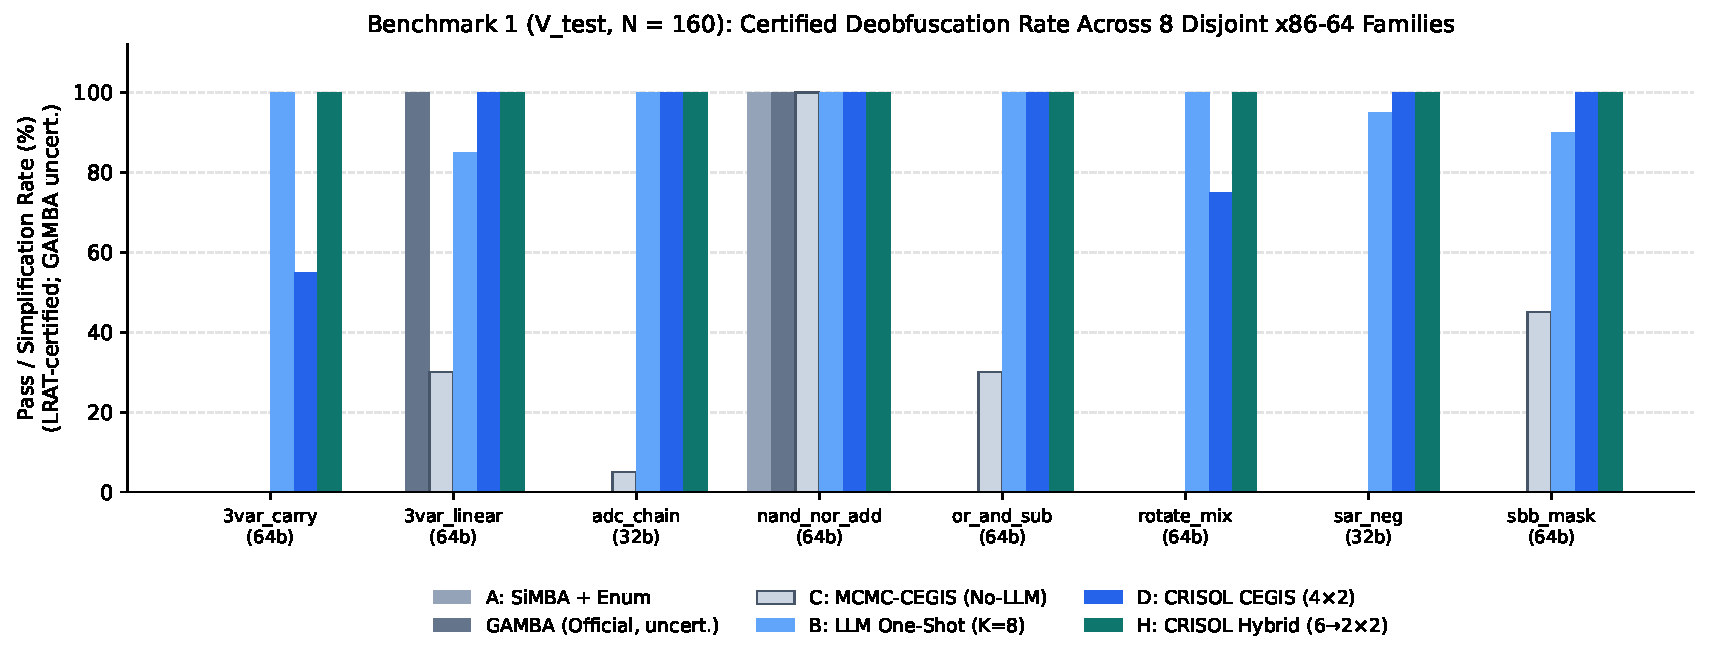
\includegraphics[width=\textwidth]{fig1_vtest_ablation.pdf}
\caption{Certified pass rates across the 8 disjoint x86-64 families of $V_{\mathrm{test}}$ ($N=160$, loop-entry 60\,s budget; under strict $\le 60.0$\,s, $C=39$, $D=145$, $H=159$).}
\label{fig:vtest}
\end{figure}

\begin{itemize}[leftmargin=1.5em]
  \item \textbf{Confirmatory $H_1$ ($D$ vs.\ $A \cup C$):} \textbf{CONFIRMED (GO)} under both cutoffs: strict $\le 60.0$\,s gives $+66.25$\,pp ($n_{10}=106, n_{01}=0$, exact McNemar $p = 2.47 \times 10^{-32} \ll 0.01$); in-flight gives $+65.00$\,pp ($n_{10}=104, n_{01}=0$, $p = 9.86 \times 10^{-32}$).
  \item \textbf{Confirmatory $H_2$ ($D$ vs.\ $B$):} \textbf{NOT CONFIRMED.} Sequential multi-round CLI latency (~20\,s/call) prevented $D$ ($145/160$ strict; $146/160$ in-flight) from surpassing One-Shot $B$ ($154/160$; exact McNemar $n_{10}=6, n_{01}=15, p = 0.078$ strict; $n_{10}=6, n_{01}=14, p = 0.115$ in-flight). Nevertheless, $D$'s counterexample feedback rescued all 6 slices where $B$ failed.
  \item \textbf{Exploratory Hybrid $H$:} Designed post-hoc after observing the negative $H_2$ latency trade-off, $H$ achieves \textbf{159/160 (99.38\%, 95\% CI $[96.6\%, 100\%]$)} under strict $\le 60.0$\,s ($+75.00$\,pp vs.\ $A \cup C$, $p = 1.50 \times 10^{-36}$; vs.\ $B$, $n_{10}=6, n_{01}=1, p = 0.125$) and \textbf{160/160 (100.0\%, 95\% CI $[97.7\%, 100\%]$)} in-flight (one slice \texttt{3var\_carry\_64\_020} finished at \textbf{74.29\,s}) in 1.01 mean LLM calls.
  \item \textbf{GAMBA domain boundary:} Official GAMBA solved \textbf{40/40 (100\%)} of the two pure-algebraic 64-bit families (\texttt{3var\_linear\_64}, \texttt{nand\_nor\_add\_64}). The remaining 120 slices (6/8 families) use x86-64 \texttt{ADC}/\texttt{SBB} carry flags, \texttt{ROL}/\texttt{ROR}, or 32$\to$64-bit zero-extension that cannot be expressed in our single-width pure-AST adapter (pure 32-bit slices without carry/rotates could be evaluated separately under GAMBA's \texttt{-b 32} mode).
  \item \textbf{Independent re-verification:} All 362/362 Phase~1 \texttt{PASS} verdicts ($A+B+C+D$) were independently re-verified (355 via \texttt{CaDiCaL} + \texttt{lrat-check} + 7 \texttt{3var\_carry\_64} slices via Lean~4 \texttt{bv\_decide} in 3.16--6.13\,s), with 0 \texttt{FAIL\_SAT} and 0 \texttt{LIFTER\_BUG}.
\end{itemize}

\subsection{Benchmark 2: Evaluating the Multiplication Certification Frontier ($V_{\mathrm{hard}}$, $N=40$)}

Table~\ref{tab:vhard} and Figure~\ref{fig:vhard} evaluate \textbf{ground-truth equivalence certification ($F_B \equiv g$)} on the 40 \texttt{IMUL} slices under an \textbf{identical 30.0\,s timeout budget across all four backends} (with at most 2 concurrent multi-threaded Lean~4 processes to prevent CPU contention). Uncertified Bitwuzla closes 40/40, Z3 \texttt{QF\_BV} closes 0/40, and raw Z3 bit-blasting + CaDiCaL LRAT closes \textbf{3/40 (7.5\%)}. \textbf{Lean 4 \texttt{bv\_decide}} raises certified proofs from \textbf{7.5\% (3/40) to 87.5\% (35/40)}.

\begin{table}[htbp]
\centering
\footnotesize
\resizebox{\textwidth}{!}{%
\begin{tabular}{@{}lrrrrr@{}}
\toprule
\textbf{Family ($n=20$ each, 30.0\,s cap)} & \textbf{Z3 \texttt{QF\_BV}} & \textbf{CaDiCaL LRAT} & \textbf{Bitwuzla (\emph{uncert.})} & \textbf{Lean 4 \texttt{bv\_decide}} & \textbf{Mean Lean 4 (all / cert.)} \\
\midrule
\texttt{test\_mba\_poly\_mul\_32} & 0 / 20 (0\%) & 3 / 20 (15\%) & 20 / 20 (100\%) & \textbf{20 / 20 (100\%)} & 5.41\,s / 5.41\,s \\
\texttt{test\_mba\_poly\_mul\_64} & 0 / 20 (0\%) & 0 / 20 (0\%) & 20 / 20 (100\%) & \textbf{15 / 20 (75\%)} & 10.57\,s / 8.70\,s \\
\midrule
\textbf{Total $V_{\mathrm{hard}}$ ($N=40$)} & \textbf{0 / 40 (0\%)} & \textbf{3 / 40 (7.5\%)} & \textbf{40 / 40 (100\%)} & \textbf{35 / 40 (87.5\%)} & \textbf{7.99\,s / 6.82\,s} \\
\bottomrule
\end{tabular}%
}
\caption{Ground-truth equivalence certification ($F_B \equiv g$) on $V_{\mathrm{hard}}$ ($N=40$ \texttt{IMUL} slices) under an equalized 30.0\,s timeout per backend.}
\label{tab:vhard}
\end{table}

\begin{figure}[htbp]
\centering
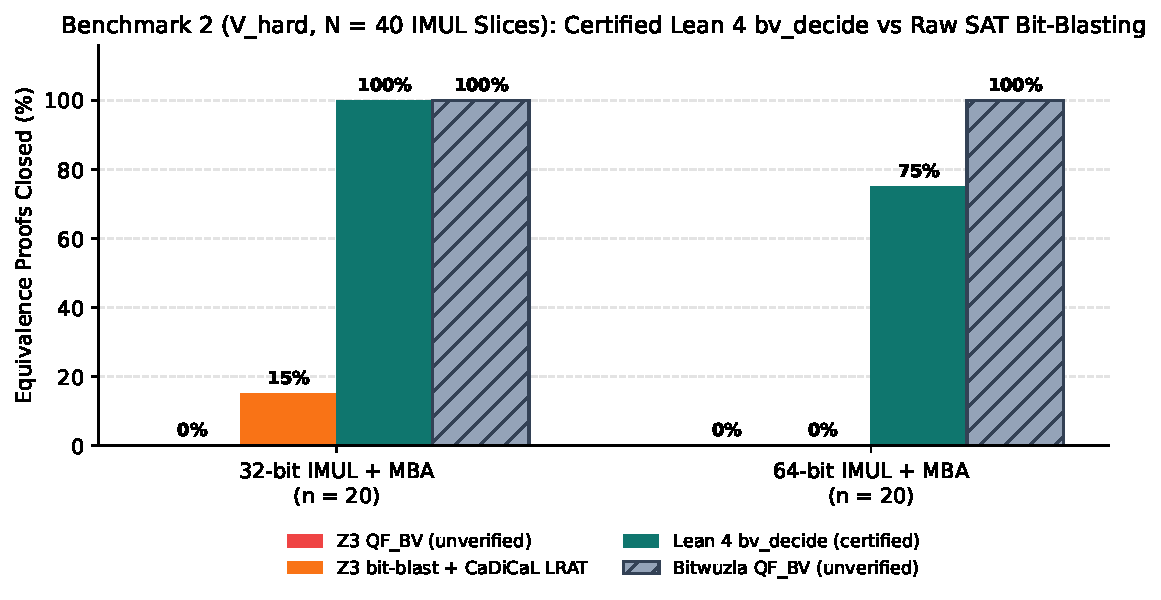
\includegraphics[width=0.78\textwidth]{fig2_vhard_lean4.pdf}
\caption{Certified proofs on $V_{\mathrm{hard}}$ under equalized 30.0\,s timeouts: Lean 4 \texttt{bv\_decide} (35/40 = 87.5\%) vs.\ raw Z3 bit-blast + CaDiCaL LRAT (3/40 = 7.5\%).}
\label{fig:vhard}
\end{figure}

\subsection{Benchmark 3: Real \texttt{gcc -O2} and \texttt{clang -O2} Compiled C Corpus ($V_{\mathrm{real}}$, $N=22$)}

Table~\ref{tab:vreal} and Figure~\ref{fig:vreal} evaluate 22 real C functions compiled with \texttt{gcc -O2} and \texttt{clang -O2} that strictly pass the 17-mnemonic allowlist (no widening). Although $A$/$C$ used LRAT while $H$ used Lean~4 \texttt{bv\_decide}, in practice $A$ and $C$ failed at the search/pre-filter stage with 0 SMT passes.

\begin{table}[htbp]
\centering
\footnotesize
\resizebox{\textwidth}{!}{%
\begin{tabular}{@{}llrrrl@{}}
\toprule
\textbf{Config} & \textbf{Oracle} & \textbf{PASS / 22} & \textbf{Rate (\%)} & \textbf{Mean (s)} & \textbf{McNemar vs.\ $A \cup C$} \\
\midrule
$A$ (SiMBA + Enum) & LRAT & 0 / 22 & 0.00 & 2.28 & --- \\
$C$ (MCMC-CEGIS) & LRAT & 0 / 22 & 0.00 & 60.02* & --- \\
\texttt{H-sol} (\texttt{gpt-6.2-sol}) & Lean 4 \texttt{bv\_decide} & 6 / 22 & 27.27 & 55.12 & $p = 0.0313$ (\emph{n.s.\ at $\alpha=0.01$}) \\
\textbf{\texttt{H-hydrogen}} (\texttt{gemini-4-hydrogen}) & \textbf{Lean 4 \texttt{bv\_decide}} & \textbf{22 / 22} & \textbf{100.00} & \textbf{23.44} & \textbf{$p = 4.77 \times 10^{-7}$} \\
\bottomrule
\end{tabular}%
}
\caption{Benchmark 3 ($V_{\mathrm{real}}$, $N=22$ real \texttt{gcc/clang -O2} compiled C functions). *60.02\,s reflects 0.02\,s loop-exit overhead past the 60\,s cap.}
\label{tab:vreal}
\end{table}

\begin{figure}[htbp]
\centering
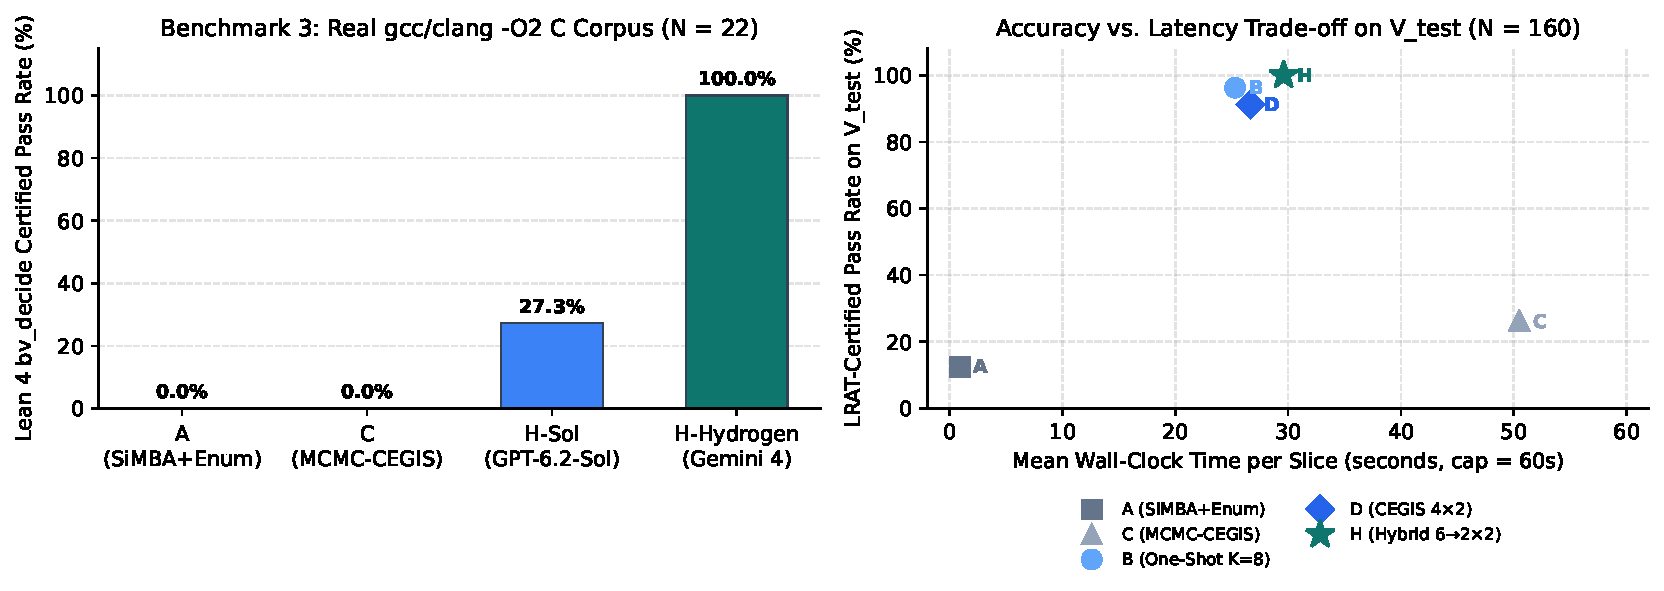
\includegraphics[width=\textwidth]{fig3_real_o2_and_tradeoff.pdf}
\caption{Left: Lean 4 \texttt{bv\_decide} certified pass rates on real \texttt{gcc/clang -O2} C binaries ($V_{\mathrm{real}}$, $N=22$). Right: accuracy vs.\ mean wall-clock latency on $V_{\mathrm{test}}$ ($N=160$).}
\label{fig:vreal}
\end{figure}

\section{Threats to Validity, Availability, and Conclusion}

\paragraph{Threats to Validity.}
Our study intentionally restricts slices to $\le 24$ straight-line, register-only instructions without memory aliasing or unbounded loops. While Lean~4 \texttt{bv\_decide} verifies bit-blasting and checks LRAT proofs inside Lean, Lean's native evaluation axiom (\texttt{<thm>.\_native.bv\_decide.ax\_*}), \texttt{oracle\_lean.py}, and our lifter (empirically verified on 82,944 three-way checks) remain in the TCB. In addition, $V_{\mathrm{real}}$ ($N=22$) draws on well-known hash and ARX primitives compiled with \texttt{gcc/clang -O2} that frontier LLMs may have encountered during pretraining; $V_{\mathrm{real}}$ therefore evaluates certified recovery across real optimizing-compiler lowerings rather than unseen algorithm discovery. Finally, integrating external commercial/academic obfuscators (Tigress, OLLVM) and open-weight local models with explicit tool-free API calls is planned for v2.

\paragraph{Code and Data Availability.}
All source code, frozen datasets, raw benchmark JSONL logs, independent re-verification logs, and an offline Artifact Evaluation script (\texttt{python3 replay\_offline.py} \texttt{--mode smoke}, requiring zero API keys) are publicly archived under the MIT License at:
\begin{itemize}[leftmargin=1.5em]
  \item \textbf{Zenodo Archive (DOI):} \url{https://doi.org/10.5281/zenodo.24476603}
  \item \textbf{GitHub Repository (tag \texttt{v1.0.0}):} \url{https://github.com/crisolabs/research-lab/tree/v1.0.0/experimentos/04-crisol-mba-x64}
\end{itemize}

\paragraph{Conclusion.}
Within straight-line x86-64 MBA deobfuscation, CRISOL-MBA-x64 confirms our pre-registered hypothesis $H_1$ ($+66.25$\,pp strict $\le 60$\,s, $p = 2.47 \times 10^{-32}$; while pre-registered $H_2$ is not confirmed due to sequential round latency), reaches 159/160 (99.38\%, 95\% CI $[96.6\%, 100\%]$) under strict $\le 60.0$\,s and 160/160 (max 74.29\,s) in-flight with exploratory Hybrid~$H$, certifies 22/22 (95\% CI $[84.6\%, 100\%]$) real \texttt{gcc/clang -O2} C functions, and raises equalized-30\,s certified \texttt{IMUL} ground-truth proofs from 7.5\% (3/40) to 87.5\% (35/40) via Lean~4 \texttt{bv\_decide} with 0 false positives relative to the declared TCB.

\bibliographystyle{plain}
\bibliography{references}

\end{document}
